\section{Modelagem do Projeto}
\subsection{Levantamento de Requisitos}
\label{sec:requisitos}

O levantamento de requisitos foi realizado por meio de uma entrevista semiestruturada com o responsável pela emissão de certificados na instituição parceira, juntamente com a observação direta do processo manual executado por ele. Durante a entrevista, foram identificadas as principais dificuldades enfrentadas, como o tempo elevado para emissão manual, a dificuldade em gerenciar grandes volumes de certificados e a ausência de um mecanismo de validação pública. A análise do processo permitiu mapear o fluxo completo de emissão, desde o cadastro de participantes até a entrega do certificado, servindo como base para a definição dos requisitos funcionais e não funcionais apresentados a seguir.


\textbf{Requisitos Funcionais}:

\subsubsection{Módulo de Autenticação e Controle de Acesso}
\begin{itemize}
\item RF001 – Permitir login por e-mail e senha.
\item RF002 – Permitir redefinição de senha via e-mail.
\item RF003 – Validar credenciais antes de conceder acesso.
\item RF004 – Permitir cadastro de novos usuários (apenas administrador).
\item RF005 – Permitir gerenciamento de perfis e permissões.
\item RF006 – Controlar acesso a áreas restritas com base no status de autenticação do usuário.
\item RF007 – Controlar sessões ativas por conta, permitindo apenas uma sessão simultânea.
\end{itemize}

\subsubsection{Módulo de Templates de Certificados}
\begin{itemize}
\item RF008 – Permitir upload de templates (PPTX, DOCX, PDF).
\item RF009 – Permitir personalização de templates.
\item RF010 – Permitir selecionar template da galeria interna.
\item RF011 – Identificar campos dinâmicos automaticamente.
\item RF012 – Permitir criação/edição manual de campos dinâmicos (ex: \{\{nome\}\}).
\item RF013 – Salvar configurações de mapeamento de campos.
\item RF014 – Permitir duplicar templates existentes.
\end{itemize}

\subsubsection{Módulo de Entrada de Dados}
\begin{itemize}
\item RF015 – Permitir cadastro individual de participantes.
\item RF016 – Permitir emissão manual para participante único.
\item RF017 – Importar dados via CSV.
\item RF018 – Importar dados via Excel (.xlsx).
\item RF019 – Configurar gatilhos de emissão automática.
\item RF020 – Permitir upload de lista em lote.
\item RF021 – Processar múltiplos certificados em fila.
\item RF022 – Notificar ao término do processamento.
\end{itemize}

\subsubsection{Módulo de Geração de Certificados}
\begin{itemize}
\item RF023 – Gerar certificados em PDF.
\item RF024 – Preencher automaticamente campos dinâmicos.
\item RF025 – Gerar código único por certificado.
\item RF026 – Registrar data, hora e localidade da emissão.
\item RF027 – Permitir reemissão mantendo histórico.
\item RF028 – Permitir download individual.
\item RF029 – Permitir download em lote.
\end{itemize}

\subsubsection{Módulo de Envio e Comunicação}
\begin{itemize}
\item RF030 – Permitir personalização do corpo do e-mail com variáveis.
\item RF031 – Registrar status de envio (pendente, enviado, falha).
\item RF032 – Reenviar automaticamente em caso de falha (até 3 tentativas a cada 10 min).
\end{itemize}

\subsubsection{Módulo de Validação Pública e Antifraude}
\begin{itemize}
\item RF033 – Disponibilizar portal público de validação.
\item RF034 – Validar certificado via código único.
\item RF035 – Gerar QR Code no certificado.
\item RF036 – Permitir personalização de cores do QR Code.
\item RF037 – Exibir informações básicas ao validar (nome, curso, data, validade, autenticidade).
\end{itemize}

\subsubsection{Módulo de Assinaturas Digitais}
\begin{itemize}
\item RF038 – Permitir adicionar assinatura digitalizada ao template.
\item RF039 – Registrar hash de verificação da assinatura.
\end{itemize}

\subsubsection{Módulo de Dashboard e Gestão}
\begin{itemize}
\item RF040 – Exibir lista completa de certificados emitidos.
\item RF041 – Permitir filtros por curso, período, status e instrutor.
\item RF042 – Exibir estatísticas mensais de emissão.
\item RF043 – Exibir logs de ações realizadas.
\end{itemize}

\subsubsection{Módulo de Auditoria e Segurança Operacional}
\begin{itemize}
\item RF044 – Registrar responsável por cada certificado gerado.
\item RF045 – Registrar data, hora e local de ações relevantes.
\item RF046 – Permitir arquivamento de certificados como alternativa à exclusão definitiva.
\end{itemize}

\subsubsection{Módulo de Gestão de Cursos/Eventos}
\begin{itemize}
\item RF047 – Permitir cadastro de cursos/eventos.
\item RF048 – Associar participantes ao curso.
\item RF049 – Definir carga horária.
\item RF050 – Registrar instrutor responsável.
\item RF051 – Configurar datas de início e término.
\item RF052 – Listar certificados vinculados ao curso.
\item RF053 – Validar vínculo do participante ao curso antes de permitir a emissão.
\item RF054 – Registrar local do curso.
\end{itemize}

\subsubsection{Módulo de Participantes}
\begin{itemize}
\item RF055 – Cadastro completo de participantes (nome, e-mail, CPF opcional).
\item RF056 – Permitir edição de dados.
\item RF057 – Importar participantes sem duplicidade.
\item RF058 – Exibir histórico de certificados por participante.
\item RF059 – Permitir busca por nome, e-mail e CPF.
\end{itemize}

\subsubsection{Módulo Multiempresa / Multi-tenant}
\begin{itemize}
\item RF060 – Permitir cadastro de múltiplas organizações.
\item RF061 – Isolar dados entre organizações.
\item RF062 – Permitir que cada empresa tenha seus próprios templates.
\item RF063 – Permitir que administradores gerenciem usuários internos.
\end{itemize}

\subsubsection{Módulo de Configurações do Sistema}
\begin{itemize}
\item RF064 – Personalizar mensagens padrão.
\item RF065 – Ativar/desativar envio automático.
\item RF066 – Configurar regras de reemissão.
\end{itemize}

\subsubsection{Módulo de Armazenamento e Arquivos}
\begin{itemize}
\item RF067 – Permitir exclusão lógica (soft-delete) de arquivos.
\item RF068 – Armazenar templates no sistema.
\end{itemize}

\subsubsection{Módulo de Notificações e Alertas}
\begin{itemize}
\item RF069 – Notificar falhas de emissão.
\item RF070 – Notificar sucesso no processamento de planilhas.
\item RF071 – Alertar quando template estiver incompleto ou inválido.
\end{itemize}

\subsubsection{Módulo de Monitoramento e Logs}
\begin{itemize}
\item RF072 – Registrar logs de autenticação e tentativas de acesso.
\item RF073 – Registrar eventos críticos (falha geração PDF etc.).
\item RF074 – Permitir exportação de logs.
\end{itemize}

\subsubsection{Módulo de Suporte, Operação e Manutenção}
\begin{itemize}
\item RF075 – Permitir abertura de chamados de suporte.
\item RF076 – Exibir status do sistema (online/manutenção).
\item RF077 – Permitir atualização de termos de uso e políticas.
\end{itemize}
\vspace{1em}
\textbf{Requisitos Não Funcionais}:

Os requisitos não funcionais foram priorizados segundo o método MoSCoW, alinhado à abordagem MVP (Produto Mínimo Viável) adotada no projeto: \textbf{[M]} \textit{Must have} — requisitos essenciais implementados no MVP; \textbf{[S]} \textit{Should have} — importantes, mas não críticos para a primeira versão; \textbf{[C]} \textit{Could have} — desejáveis para versões futuras; \textbf{[W]} \textit{Won't have} — fora do escopo do MVP.

\subsubsection{Segurança}
\begin{itemize}
\rnfitem{rnf:supabase-auth}{[S] O sistema deve utilizar o Supabase Auth para gerenciamento seguro de autenticação e armazenamento de senhas com hash criptográfico seguro (bcrypt).}
\rnfitem{rnf:https}{[M] O sistema deve utilizar conexão segura HTTPS (TLS 1.2 ou superior) em todas as comunicações entre o cliente e o servidor, garantindo confidencialidade e integridade dos dados em trânsito.}
\rnfitem{rnf:encryption-at-rest}{[S] O sistema deve proteger dados sensíveis em repouso utilizando criptografia fornecida pela infraestrutura em nuvem.}
\rnfitem{rnf:login-attempt-limit}{[S] O sistema deve bloquear autenticação após 5 tentativas consecutivas inválidas (conforme política do provedor de autenticação).}
\rnfitem{rnf:session-timeout}{[C] Sessões inativas devem expirar automaticamente após tempo configurável (ex.: 30 minutos).}
\rnfitem{rnf:rbac}{[M] O sistema deve implementar controle de acesso baseado em papéis (RBAC).}
\rnfitem{rnf:owasp}{[S] O sistema deve seguir boas práticas de segurança conforme OWASP Top 10.}
\rnfitem{rnf:auth-logs}{[S] O sistema deve registrar logs de autenticação e eventos de segurança, incluindo tentativas de login, falhas, acessos negados e alterações de configuração, com data, hora e identificação do usuário.}
\rnfitem{rnf:tenant-isolation}{[C] O sistema deve garantir isolamento de dados entre empresas (multi-tenant).}
\rnfitem{rnf:mfa}{[W] O sistema deve permitir futura implementação de autenticação multifator (MFA).}
\rnfitem{rnf:emission-schedules}{[C] O sistema deve permitir configurar horários de emissão por perfil de colaborador como política de segurança.}
\end{itemize}

\subsubsection{Desempenho e Escalabilidade}

Os valores numéricos apresentados a seguir são estimativas definidas pelo desenvolvedor com base no porte esperado da operação, considerando turmas típicas de 20 a 50 participantes, palestras com até 200 participantes e emissões recorrentes ao longo do ano. Os limites estabelecidos consideram uma margem de segurança para absorver picos sazonais sem degradação da experiência do usuário.

\vspace{0.5em}
\begin{itemize}
\rnfitem{rnf:batch-capacity}{[M] O sistema deve suportar geração simultânea de, estimados, 500 certificados por lote, volume equivalente a duas turmas grandes ou dez turmas médias processadas em única operação.}
\rnfitem{rnf:generation-time}{[M] O tempo médio de geração individual não deve exceder 5 segundos por certificado, garantindo que um lote de 500 certificados seja concluído em aproximadamente 42 minutos.}
\rnfitem{rnf:validation-response-time}{[M] O portal público de validação deve responder em até 2 segundos.}
\rnfitem{rnf:horizontal-scaling}{[S] O sistema deve permitir escalabilidade horizontal do serviço de geração.}
\rnfitem{rnf:monthly-volume}{[S] O sistema deve suportar volume estimado de 10.000 certificados/mês, compatível com a projeção de emissões recorrentes acrescida de margem de segurança.}
\rnfitem{rnf:async-batch-processing}{[M] A geração em lote deve ser processada de forma assíncrona por meio de fila de processamento, sem bloquear a aplicação principal.}
\rnfitem{rnf:queue-ordering}{[S] A fila de certificados deve garantir processamento ordenado e controle de concorrência.}
\end{itemize}

\subsubsection{Disponibilidade e Confiabilidade}
\begin{itemize}
\rnfitem{rnf:uptime}{[S] O sistema deve garantir disponibilidade mínima de 99,5\% mensal.}
\rnfitem{rnf:daily-backup}{[S] O sistema deve realizar backup automático diário do banco de dados, com retenção mínima de 30 dias, garantindo recuperação de dados em caso de falha ou corrupção.}
\rnfitem{rnf:restore-time}{[C] O sistema deve permitir restauração de dados em até 24 horas.}
\rnfitem{rnf:retry-mechanism}{[S] O sistema deve implementar mecanismo de retentativa automática para tarefas falhas na fila de certificados.}
\rnfitem{rnf:failure-logging}{[M] O sistema deve registrar falhas de processamento para auditoria posterior.}
\end{itemize}

\subsubsection{Usabilidade e Acessibilidade}
\begin{itemize}
\rnfitem{rnf:responsive}{[M] O sistema deve ser responsivo (desktop, tablet e mobile).}
\rnfitem{rnf:visual-consistency}{[M] O sistema deve manter padrão visual consistente.}
\rnfitem{rnf:error-messages}{[M] O sistema deve fornecer mensagens de erro claras.}
\rnfitem{rnf:keyboard-nav}{[S] O sistema deve permitir navegação por teclado.}
\rnfitem{rnf:wcag}{[C] O sistema deve seguir recomendações WCAG 2.1 nível AA (quando aplicável).}
\end{itemize}

\subsubsection{Compatibilidade e Integração}
\begin{itemize}
\rnfitem{rnf:browser-compat}{[M] O sistema deve ser compatível com navegadores modernos (Chrome, Firefox, Edge, Safari).}
\rnfitem{rnf:pdf-fidelity}{[M] A geração de PDF deve preservar fidelidade visual do template original.}
\rnfitem{rnf:rest-api}{[M] O sistema deve disponibilizar API REST autenticada via token JWT do Supabase.}
\rnfitem{rnf:csv-utf8}{[S] O sistema deve aceitar arquivos CSV codificados em UTF-8.}
\rnfitem{rnf:webhooks}{[C] O sistema deve permitir integração via Webhooks em formato JSON.}
\end{itemize}

\subsubsection{Armazenamento e Retenção}
\begin{itemize}
\rnfitem{rnf:storage-retention}{[S] O sistema deve armazenar certificados de forma permanente, garantindo validação indefinida pelo portal público.}
\rnfitem{rnf:soft-delete}{[S] O sistema deve aplicar exclusão lógica (soft delete) quando aplicável.}
\end{itemize}

\subsubsection{Conformidade Legal e LGPD}
\begin{itemize}
\rnfitem{rnf:lgpd}{[C] O sistema deve estar em conformidade com a LGPD (Lei nº 13.709/2018), garantindo tratamento adequado dos dados pessoais coletados, incluindo consentimento, finalidade específica, minimização de dados e direitos do titular.}
\rnfitem{rnf:data-deletion}{[C] O sistema deve permitir exclusão ou anonimização de dados pessoais mediante solicitação.}
\rnfitem{rnf:consent-logging}{[C] O sistema deve registrar consentimento do usuário para o tratamento de dados pessoais, incluindo finalidade, base legal e data da coleta.}
\rnfitem{rnf:sensitive-logs}{[S] Logs sensíveis devem ser acessíveis apenas por administradores autorizados.}
\rnfitem{rnf:audit-trail}{[S] O sistema deve manter trilha de auditoria inviolável para operações críticas.}
\end{itemize}

\subsubsection{Arquitetura e Tecnologia}
\begin{itemize}
\rnfitem{rnf:independent-apps}{[M] O sistema deve ser composto por duas aplicações independentes: uma \textit{Single Page Application} (SPA) para o frontend e uma API REST para o backend, cada uma com seu próprio ciclo de vida de desenvolvimento e deploy.}
\rnfitem{rnf:frontend-layers}{[M] O frontend deve adotar arquitetura em camadas com React, com quatro camadas: (i) \textit{View} --- componentes de interface; (ii) \textit{ViewModel} --- custom hooks que encapsulam estado e ações; (iii) \textit{Service} --- cliente de comunicação com a API; (iv) \textit{Model} --- interfaces TypeScript que definem as entidades de domínio.}
\rnfitem{rnf:backend-layers}{[M] O backend deve adotar arquitetura em camadas (domínio, aplicação e infraestrutura), com as dependências apontando para a camada de domínio (princípio de inversão de dependências).}
\rnfitem{rnf:api-communication}{[M] A comunicação entre frontend e backend deve ocorrer exclusivamente via API REST sobre HTTPS, com autenticação baseada em token JWT.}
\rnfitem{rnf:async-cert-generation}{[S] A geração de certificados em lote deve ser processada de forma assíncrona por meio de fila de processamento, sem bloquear a aplicação principal.}
\rnfitem{rnf:postgresql}{[M] O sistema deve utilizar banco de dados relacional com integridade referencial (PostgreSQL), gerenciado pelo Supabase.}
\rnfitem{rnf:multi-tenant-strategy}{[C] O sistema deve implementar estratégia de isolamento multi-tenant (por schema ou coluna organizacional).}
\rnfitem{rnf:monitoring}{[S] O sistema deve implementar monitoramento e observabilidade centralizada (logs, métricas e rastreamento).}
\rnfitem{rnf:static-deploy}{[M] O frontend deve ser compilado como site estático e implantado em plataforma de hospedagem com deploy contínuo a partir do repositório Git.}
\rnfitem{rnf:backend-deploy}{[M] O backend deve ser implantado como serviço web independente em plataforma em nuvem compatível com Node.js.}
\rnfitem{rnf:extensibility}{[S] O sistema deve permitir extensibilidade, garantindo que novos módulos possam ser adicionados seguindo os mesmos padrões arquiteturais já estabelecidos.}
\end{itemize}

\subsubsection{Manutenção e Monitoramento}
\begin{itemize}
\rnfitem{rnf:zero-downtime-deploy}{[S] O sistema deve permitir atualização com mínima indisponibilidade (deploy contínuo).}
\rnfitem{rnf:documentation}{[M] O sistema deve possuir documentação técnica e manual do usuário.}
\rnfitem{rnf:error-monitoring}{[S] O sistema deve registrar erros em sistema centralizado de monitoramento.}
\rnfitem{rnf:backward-compatibility}{[S] O sistema deve permitir extensibilidade sem impacto nas funcionalidades existentes.}
\rnfitem{rnf:template-history}{[C] O sistema deve manter histórico de versões de templates, configurações e endpoints da API para fins de auditoria, rastreabilidade e versionamento.}
\end{itemize}

\subsubsection{Internacionalização}
\begin{itemize}
\rnfitem{rnf:timezone}{[S] O sistema deve permitir configuração de timezone por organização.}
\rnfitem{rnf:i18n}{[W] O sistema deve permitir tradução futura da interface.}
\rnfitem{rnf:date-format}{[C] O sistema deve suportar diferentes formatos de data e hora.}
\end{itemize}

\subsection{Regras de Negócio}

Além dos requisitos funcionais, foram identificadas regras de negócio que impõem restrições ou condições sobre as funcionalidades do sistema:

\begin{itemize}
\rnitem{rn:acesso-restrito}{Não deve ser permitido acesso a áreas restritas sem autenticação prévia.}
\rnitem{rn:certificado-arquivado}{Certificados não podem ser excluídos definitivamente, devendo ser arquivados.}
\rnitem{rn:vinculo-participante}{Certificados só podem ser emitidos para participantes previamente vinculados ao curso ou evento.}
\rnitem{rn:reenvio-limite}{O reenvio automático de certificados com falha deve respeitar o limite máximo de 3 tentativas com intervalo mínimo de 10 minutos entre cada uma.}
\end{itemize}

\subsubsection{Status de Implementação das Regras de Negócio}

As regras de negócio acima representam o modelo completo desejado para o sistema. No entanto, considerando o escopo do MVP (v1.0), algumas regras ainda não foram implementadas:

\begin{itemize}
\item \textbf{rn:certificado-arquivado} --- No MVP atual, a exclusão de templates e certificados é realizada por exclusão definitiva (\textit{hard delete}), conforme testado nos casos CT005 e CT056 do plano de testes. A regra de arquivamento (\textit{soft delete}) está prevista para a versão 2.0, conforme o requisito \ref{rf:arquivamento-certificados} [S].
\item \textbf{rn:vinculo-participante} --- A validação de vínculo entre participante e curso não é verificada no MVP, pois as entidades Participantes e Cursos ainda não foram materializadas no banco de dados.
\item \textbf{rn:reenvio-limite} --- O reenvio automático com limite de tentativas não foi implementado no MVP; o envio de e-mails é simulado sem controle de retentativas.
\end{itemize}

A implementação completa dessas regras está vinculada aos requisitos classificados como [S] ou [C], que serão tratados em versões futuras do sistema.


\subsection{Critérios de Aceitação}

Cada requisito funcional possui critérios de aceitação que definem as condições necessárias para considerá-lo atendido. A Tabela~\ref{tab:criterios} apresenta os critérios para todos os RFs.

\renewcommand{\arraystretch}{0.9}
\small
\begin{longtable}{p{1cm} p{3.2cm} p{10.8cm}}
\caption{Critérios de aceitação dos requisitos funcionais}
\label{tab:criterios}\\
\toprule
\textbf{RF} & \textbf{Descrição} & \textbf{Critério de Aceitação} \\
\midrule
\endfirsthead
\toprule
\textbf{RF} & \textbf{Descrição} & \textbf{Critério de Aceitação} \\
\midrule
\endhead
\bottomrule
\endfoot
\bottomrule
\endlastfoot
RF001 & Login por e-mail e senha & Usuário com credenciais válidas acessa o sistema; credenciais inválidas exibem mensagem de erro sem redirecionar. \\
RF002 & Redefinição de senha & Usuário clica em "Esqueci senha", insere e-mail e recebe link de redefinição válido por 1 hora. \\
RF003 & Validar credenciais & Rotas protegidas redirecionam para login quando o usuário não está autenticado; API retorna 401 para requisições sem token. \\
RF004 & Cadastro de usuários & Apenas administrador pode acessar tela de cadastro; formulário exige nome, e-mail e senha; usuário criado aparece na lista. \\
RF005 & Gerenciar perfis & Administrador pode listar, criar, editar e desativar usuários; alterações persistem após recarregar. \\
RF006 & Controle de acesso & Usuário não autenticado é redirecionado para login ao acessar qualquer rota administrativa. \\
RF007 & Sessão única & Login em novo dispositivo invalida sessão anterior; sessão expira após 30 min de inatividade. \\
\midrule
RF008 & Upload de templates & Arquivos .pptx e .pdf são aceitos; formatos .exe, .zip são rejeitados com mensagem clara; template aparece na galeria após upload. \\
RF009 & Personalização & Cores, fontes e bordas configuradas são refletidas no preview visual. \\
RF010 & Selecionar template & Galeria exibe templates salvos com nome e preview; seleção carrega o template para edição. \\
RF011 & Identificar campos automáticos & Sistema sugere campos \{\{nome\}\}, \{\{curso\}\} ao fazer upload; sugestões são editáveis. \\
RF012 & Criar/editar campos & Usuário adiciona campo \{\{cpf\}\}, salva, e o campo aparece na tela de emissão. \\
RF013 & Salvar configurações & Mapeamento de campos persiste após recarregar a página. \\
RF014 & Duplicar templates & Duplicata cria cópia idêntica com nome "(cópia)"; original não é alterado. \\
\midrule
RF015 & Cadastro individual & Formulário válido salva participante; e-mail duplicado exibe alerta; participante aparece na lista. \\
RF016 & Emissão manual & Selecionar template, preencher dados e confirmar gera certificado listado no dashboard. \\
RF017 & Importar CSV & Arquivo CSV com cabeçalho correto importa participantes; linhas com erro são ignoradas e reportadas. \\
RF018 & Importar Excel & Arquivo .xlsx com abas é processado; primeira aba é usada como padrão. \\
RF019 & Gatilhos automáticos & Ao cadastrar participante em curso com gatilho ativo, certificado é emitido automaticamente em até 30s. \\
RF020 & Upload em lote & Arquivo com 100 participantes é processado; certificados são gerados para todos. \\
RF021 & Fila de processamento & Lote de 500 participantes é enfileirado; barra de progresso mostra andamento. \\
RF022 & Notificar término & Processamento concluído envia notificação na tela (toast) com resumo. \\
\midrule
RF023 & Gerar PDF & PDF gerado preserva layout, cores e fontes do template; campos preenchidos aparecem nas posições corretas; geração leva menos de 5 segundos. \\
RF024 & Preencher campos & Dados do participante substituem corretamente os \{\{placeholders\}\} no PDF. \\
RF025 & Código único & Cada certificado possui código único (UUID v4); consulta no banco retorna apenas um registro. \\
RF026 & Data/hora/local & Certificado exibe data e hora da emissão; localização é definida pelo curso ou configuração. \\
RF027 & Reemissão & Reemissão gera novo PDF com novo código; histórico lista versão anterior com data. \\
RF028 & Download individual & PDF é baixado com nome no formato \texttt{Nome\_Curso\_Data.pdf}. \\
RF029 & Download em lote & Selecionar múltiplos certificados e baixar gera arquivo .zip com todos os PDFs. \\
\midrule
RF030 & Personalizar e-mail & Variáveis \{\{nome\}\}, \{\{link\}\} são substituídas no corpo do e-mail enviado. \\
RF031 & Status de envio & Certificado exibe status "Pendente", "Enviado" ou "Falha"; status é atualizado em tempo real. \\
RF032 & Reenvio automático & Falha de envio dispara nova tentativa após 10 min, até 3 tentativas. \\
\midrule
RF033 & Portal de validação & URL pública \texttt{/validar} exibe campo para inserir código; página é responsiva. \\
RF034 & Validar via código & Código válido exibe dados do certificado; inválido mostra "Certificado não encontrado". \\
RF035 & QR Code & QR Code no PDF redireciona para URL de validação com código como parâmetro. \\
RF036 & Exibir informações & Tela de validação mostra nome, curso, data, carga horária e status "Autêntico". \\
\midrule
RF037 & Assinatura digitalizada & Imagem de assinatura aparece na posição configurada no template. \\
RF038 & Hash da assinatura & Hash SHA-256 da assinatura é armazenado e verificável. \\
\midrule
RF039 & Lista de certificados & Tabela exibe certificados com colunas: nome, curso, data, status; paginação de 20 itens. \\
RF040 & Filtros & Filtrar por curso, período, status e instrutor atualiza a tabela sem recarregar a página. \\
RF041 & Estatísticas mensais & Dashboard exibe total de emissões por mês em gráfico de barras; dados são atualizados automaticamente. \\
RF042 & Logs de ações & Tabela de logs exibe ação, usuário, data e detalhes; ordenada por data decrescente. \\
\midrule
RF043 & Responsável & Certificado gerado registra ID do usuário que emitiu; exibido no histórico. \\
RF044 & Data/hora ações & Toda ação de emissão, edição e exclusão registra timestamp. \\
RF045 & Arquivamento & Certificado arquivado não aparece na lista padrão, mas é recuperável via filtro "Arquivados". \\
\midrule
RF046 & Cadastro cursos & Formulário salva nome, tipo, carga horária, datas e instrutor; curso aparece na lista. \\
RF047 & Associar participantes & Participante é vinculado ao curso no momento da emissão. \\
RF048 & Carga horária & Carga horária definida no curso aparece no campo correspondente do certificado. \\
RF049 & Instrutor & Nome do instrutor é salvo e exibido no certificado. \\
RF050 & Configurar datas & Datas configuradas são preenchidas automaticamente no certificado. \\
RF051 & Listar por curso & Filtro "Curso" exibe apenas certificados daquele curso. \\
RF052 & Validar vínculo & Emissão é bloqueada se participante não pertence ao curso selecionado; mensagem exibe motivo. \\
RF053 & Registrar local & Local do curso é salvo e exibido no certificado. \\
\midrule
RF054 & Cadastro completo & Nome e e-mail são obrigatórios; CPF é opcional; e-mail inválido é rejeitado. \\
RF055 & Edição & Dados editados são salvos e refletidos na tela de emissão. \\
RF056 & Importar sem duplicidade & Mesmo CPF/e-mail não cria registro duplicado; dados existentes são atualizados. \\
RF057 & Histórico & Página do participante exibe todos os certificados emitidos para ele. \\
RF058 & Busca & Busca por nome retorna resultados em menos de 2s; busca vazia retorna lista completa. \\
\midrule
RF059 & Cadastro organizações & Formulário salva CNPJ, razão social e contato; organização aparece na lista. \\
RF060 & Associar user/org & Usuário é vinculado a uma organização no cadastro; vínculo é editável. \\
RF061 & Templates por org & Organização A não vê templates da organização B. \\
RF062 & Usuários por org & Organização A não vê usuários da organização B. \\
\midrule
RF063 & Mensagens padrão & Texto padrão de e-mail é configurável por organização. \\
RF064 & Envio automático & Opção "Enviar automaticamente" é ativável/desativável por organização. \\
RF065 & Regras de reemissão & Reemissão é permitida apenas se configurada; limite de reemissões é respeitado. \\
\midrule
RF066 & Armazenar templates & Template enviado fica imediatamente disponível para uso; download do template original é possível. \\
\midrule
RF067 & Notificar falhas & Falha de emissão dispara notificação ao administrador com detalhes do erro. \\
RF068 & Notificar sucesso & Processamento concluído com sucesso exibe toast com total de certificados. \\
RF069 & Alertar template inválido & Template sem campos \{\{nome\}\} exibe alerta antes da emissão. \\
\midrule
RF070 & Logs de autenticação & Tentativa de login com senha incorreta é registrada com timestamp e IP. \\
RF071 & Eventos críticos & Falha de geração de PDF é registrada com stack trace e ID do certificado. \\
RF072 & Exportar logs & Logs são exportáveis em CSV com filtro por período. \\
\midrule
RF073 & Chamados de suporte & Formulário de chamado salva descrição, prioridade e contato; chamado é listado. \\
RF074 & Status do sistema & Página de status exibe "Online", "Em manutenção" ou "Indisponível". \\
RF075 & Termos de uso & Atualização de termos exibe aviso para aceite na próxima autenticação. \\
\bottomrule
\end{longtable}
\normalsize
\renewcommand{\arraystretch}{1.0}


\subsection{Matriz de Rastreabilidade}

O Quadro~\ref{qua:rastreabilidade} apresenta a matriz de rastreabilidade que relaciona os requisitos funcionais implementados no MVP aos casos de uso, às principais classes do diagrama de classes e às tabelas do banco de dados, garantindo a rastreabilidade entre os artefatos do projeto. A tabela foi disposta em orientação vertical (rotacionada 90\textdegree) para preservar a legibilidade de seu conteúdo, uma vez que possui quatro colunas com textos extensos.

\clearpage
\begingroup
\renewcommand{\tablename}{Quadro}
\begin{sidewaystable}[p!]
\centering
\footnotesize
\captionsetup{type=quadro}
\caption{Matriz de rastreabilidade entre requisitos funcionais, casos de uso, classes e tabelas implementados no MVP}
\label{qua:rastreabilidade}
\setlength{\tabcolsep}{3pt}
\renewcommand{\arraystretch}{0.9}
\begin{tabularx}{\textwidth}{|>{\raggedright\arraybackslash}X|>{\raggedright\arraybackslash}X|>{\raggedright\arraybackslash}X|>{\raggedright\arraybackslash}X|}
\hline
\textbf{Módulo / RFs} & \textbf{Casos de Uso} & \textbf{Classes} & \textbf{Tabelas} \\
\hline
Templates de Certificados (\ref{rf:upload-templates}–\ref{rf:mapeamento-campos}) & Gerenciar Templates (UC002), Criar Template, Editar Template, Salvar Template & Template, TemplateLayout & TEMPLATES \\
\hline
Entrada de Dados e Emissão (\ref{rf:cadastro-participante}, \ref{rf:emissao-manual}) & Emitir Certificado Individual (UC004) & Certificate, EmitCertificateUseCase, ICertificateRepository & CERTIFICADOS \\
\hline
Geração de Certificados (\ref{rf:gerar-pdf}–\ref{rf:download-individual}) & Emitir Certificado (UC004), Gerar PDF, Obter Certificado & Certificate, VerificationCode, EmitCertificateUseCase, GeneratePDFUseCase, GetCertificateUseCase, ICertificateRepository, ITemplateRepository, IPDFService, SupabaseCertificateRepository, SupabaseTemplateRepository, PDFKitService & CERTIFICADOS \\
\hline
Validação Pública (\ref{rf:portal-validacao}–\ref{rf:exibir-validacao}) & Validar Certificado (UC008) & VerifyCertificateUseCase, VerifyResult, Certificate (Frontend) & CERTIFICADOS \\
\hline
Dashboard e Gestão (\ref{rf:lista-certificados}–\ref{rf:estatisticas-emissao}) & Visualizar Dashboard (UC014) & Certificate (Frontend), Template (Frontend) & CERTIFICADOS, TEMPLATES \\
\hline
Armazenamento de Templates (\ref{rf:armazenar-templates}) & Gerenciar Templates (UC002) & Template, SupabaseTemplateRepository & TEMPLATES \\
\hline
\end{tabularx}
\end{sidewaystable}
\par\vspace{4pt}
\begin{center}\small\textit{Fonte: Elaborado pelo Autor (2026).}\end{center}
\endgroup
\clearpage


\subsection{Diagramas de casos de uso}
\begin{figure}[H]
\centering
\resizebox{\textwidth}{!}{
\begin{tikzpicture}[
    scale=0.7,
    transform shape,
    actor/.style={rectangle, draw=black, fill=blue!20, rounded corners, minimum width=1.8cm, minimum height=0.7cm},
    usecase/.style={ellipse, draw=black, minimum width=2.5cm, minimum height=0.8cm, font=\small},
    include/.style={->, dashed, font=\tiny},
    assoc/.style={-},
    every node/.style={font=\small}
]

% Fronteira do sistema
\draw (-0.5,-8.5) rectangle (18,5) node[above left, font=\small\bfseries, inner sep=3pt] at (18,5) {Sistema de Certificados};

% Atores
\node[actor] (admin) at (-3,1.5) {Administrador};
\node[actor] (colab) at (-3,-1.5) {Colaborador};
\node[actor] (visit) at (-3,-5) {Visitante};

% Generalização: Administrador herda casos de uso do Colaborador
\draw[-{Triangle[open]}] (admin) -- (colab);

% Casos Admin
\node[usecase, fill=red!20] (usuarios) at (2.5,3.5) {Gerenciar Usuários};
\node[usecase, fill=red!20] (template) at (2.5,1.8) {Criar Template};
\node[usecase, fill=red!20] (cursos) at (2.5,0) {Gerenciar Cursos};

\node[usecase, fill=yellow!30] (permissoes) at (7.5,3.5) {Definir Permissões};
\node[usecase, fill=red!20] (campos) at (7.5,1.8) {Configurar Campos};
\node[usecase, fill=red!20] (editar) at (7.5,0) {Editar Template};

\node[usecase, fill=yellow!30] (salvar) at (12,1.8) {Salvar};
\node[usecase, fill=yellow!30] (preview) at (16,0) {Prévia};

% Casos Colaborador
\node[usecase, fill=green!30] (emitir) at (2.5,-1.5) {Emitir Individual};
\node[usecase, fill=green!30] (lote) at (2.5,-3) {Emitir em Lote};
\node[usecase, fill=orange!40] (cadastro) at (2.5,-4.2) {Cadastrar Part.};
\node[usecase, fill=orange!40] (importar) at (2.5,-5.2) {Importar Part.};

\node[usecase, fill=purple!25] (pdf) at (7.5,-1.5) {Gerar PDF};
\node[usecase, fill=purple!25] (codigo) at (11,-1.5) {Gerar Código};
\node[usecase, fill=purple!25] (registro) at (14.5,-1.5) {Registrar};

\node[usecase, fill=purple!25] (fila) at (7.5,-3) {Fila};
\node[usecase, fill=purple!25] (notificar) at (11,-3) {Notificar};
\node[usecase, fill=purple!25] (email) at (14.5,-3) {Email};

\node[usecase, fill=blue!30] (validardados) at (7.5,-5.2) {Validar Dados};

% Casos Visitante
\node[usecase, fill=red!20] (validar) at (2.5,-6.8) {Validar Cert.};
\node[usecase, fill=blue!30] (consultar) at (7.5,-6.8) {Consultar Cód.};
\node[usecase, fill=blue!30] (dados) at (11,-6.8) {Exibir Dados};

% Associações
\draw[assoc] (admin) -- (usuarios);
\draw[assoc] (admin) -- (template);
\draw[assoc] (admin) -- (cursos);
\draw[assoc] (admin) -- (emitir);

\draw[assoc] (colab) -- (emitir);
\draw[assoc] (colab) -- (lote);
\draw[assoc] (colab) -- (cadastro);
\draw[assoc] (colab) -- (importar);

\draw[assoc] (visit) -- (validar);

% Includes
\draw[include] (usuarios) -- (permissoes);
\draw[include] (template) -- (campos);
\draw[include] (template) -- (editar);
\draw[include] (campos) -- (salvar);
\draw[include] (editar) -- (salvar);
\draw[include] (salvar) -- (preview);

\draw[include] (emitir) -- (pdf);
\draw[include] (pdf) -- (codigo);
\draw[include] (codigo) -- (registro);
\draw[include] (registro) -- (email);

\draw[include] (lote) -- (fila);
\draw[include] (fila) -- (notificar);

\draw[include] (importar) -- (validardados);

\draw[include] (validar) -- (consultar);
\draw[include] (consultar) -- (dados);

\end{tikzpicture}
}
\caption{Diagrama de casos de uso do sistema de certificados}
\label{fig:casos-uso}
\end{figure}


A Tabela~\ref{tab:uc001} ao \ref{tab:uc008} apresentam as descrições textuais dos casos de uso identificados no diagrama da Figura~\ref{fig:casos-uso}.

\begin{table}[H]
\centering
\small
\setlength{\tabcolsep}{4pt}
\begin{tabular}{p{3cm} p{12cm}}
\toprule
\textbf{Caso de Uso} & UC001 -- Gerenciar Usuários \\
\midrule
\textbf{Ator} & Administrador \\
\midrule
\textbf{Pré-condições} & Administrador autenticado no sistema. \\
\midrule
\textbf{Fluxo Principal} & 1. Administrador acessa a seção de usuários. \\
 & 2. Sistema exibe lista de usuários cadastrados. \\
 & 3. Administrador seleciona criar, editar ou desativar um usuário. \\
 & 4. Sistema valida e persiste a alteração. \\
 & 5. Sistema exibe confirmação. \\
\midrule
\textbf{Fluxo Alternativo} & \textbf{FA01 — Definir permissões:} durante a edição, o administrador pode definir perfis de acesso do usuário. \\
\midrule
\textbf{Fluxo de Exceção} & \textbf{FE01 — E-mail duplicado:} sistema rejeita cadastro e exibe mensagem. \\
\midrule
\textbf{Pós-condições} & Usuário criado/editado/desativado com sucesso; alterações refletidas na lista. \\
\bottomrule
\end{tabular}
\caption{Descrição do caso de uso UC001 -- Gerenciar Usuários}
\label{tab:uc001}
\end{table}

\begin{table}[H]
\centering
\small
\setlength{\tabcolsep}{4pt}
\begin{tabular}{p{3cm} p{12cm}}
\toprule
\textbf{Caso de Uso} & UC002 -- Gerenciar Templates \\
\midrule
\textbf{Ator} & Administrador \\
\midrule
\textbf{Pré-condições} & Administrador autenticado. \\
\midrule
\textbf{Fluxo Principal} & 1. Administrador acessa a seção de templates. \\
 & 2. Sistema exibe galeria de templates existentes. \\
 & 3. Administrador faz upload de novo arquivo PPTX. \\
 & 4. Sistema valida o formato e exibe preview. \\
 & 5. Administrador configura campos dinâmicos (\{\{nome\}\}, \{\{curso\}\}, etc.) e personaliza cores e fontes. \\
 & 6. Administrador salva o template. \\
\midrule
\textbf{Fluxo Alternativo} & \textbf{FA01 — Editar template:} administrador seleciona template existente, altera configurações e salva. \\
\midrule
\textbf{Fluxo de Exceção} & \textbf{FE01 — Formato inválido:} arquivo diferente de PPTX é rejeitado. \\
\bottomrule
\textbf{Pós-condições} & Template salvo e disponível para uso na emissão de certificados. \\
\bottomrule
\end{tabular}
\caption{Descrição do caso de uso UC002 -- Gerenciar Templates}
\label{tab:uc002}
\end{table}

\begin{table}[H]
\centering
\small
\setlength{\tabcolsep}{4pt}
\begin{tabular}{p{3cm} p{12cm}}
\toprule
\textbf{Caso de Uso} & UC003 -- Gerenciar Cursos \\
\midrule
\textbf{Ator} & Administrador \\
\midrule
\textbf{Pré-condições} & Administrador autenticado. \\
\midrule
\textbf{Fluxo Principal} & 1. Administrador acessa seção de cursos. \\
 & 2. Sistema exibe lista de cursos cadastrados. \\
 & 3. Administrador preenche nome, carga horária, datas e instrutor. \\
 & 4. Sistema valida e salva o curso. \\
 & 5. Sistema exibe confirmação. \\
\midrule
\textbf{Fluxo de Exceção} & \textbf{FE01 — Dados obrigatórios ausentes:} sistema bloqueia salvamento até preenchimento. \\
\midrule
\textbf{Pós-condições} & Curso cadastrado e disponível para vinculação com certificados. \\
\bottomrule
\end{tabular}
\caption{Descrição do caso de uso UC003 -- Gerenciar Cursos}
\label{tab:uc003}
\end{table}

\begin{table}[H]
\centering
\small
\setlength{\tabcolsep}{4pt}
\begin{tabular}{p{3cm} p{12cm}}
\toprule
\textbf{Caso de Uso} & UC004 -- Emitir Certificado Individual \\
\midrule
\textbf{Ator} & Colaborador \\
\midrule
\textbf{Pré-condições} & Colaborador autenticado; template e curso cadastrados. \\
\midrule
\textbf{Fluxo Principal} & 1. Colaborador acessa a seção de emissão. \\
 & 2. Sistema exibe formulário com template, curso e participante. \\
 & 3. Colaborador seleciona template, curso e participante. \\
 & 4. Sistema valida vínculo do participante ao curso. \\
 & 5. Sistema gera PDF preenchendo campos dinâmicos. \\
 & 6. Sistema gera código único e QR Code. \\
 & 7. Sistema registra data, hora e responsável. \\
 & 8. Sistema exibe certificado gerado com opção de download. \\
\midrule
\textbf{Fluxo de Exceção} & \textbf{FE01 — Participante sem vínculo:} sistema bloqueia emissão e exibe alerta. \\
\midrule
\textbf{Pós-condições} & Certificado gerado, código único registrado e disponível para validação pública. \\
\bottomrule
\end{tabular}
\caption{Descrição do caso de uso UC004 -- Emitir Certificado Individual}
\label{tab:uc004}
\end{table}

\begin{table}[H]
\centering
\small
\setlength{\tabcolsep}{4pt}
\begin{tabular}{p{3cm} p{12cm}}
\toprule
\textbf{Caso de Uso} & UC005 -- Emitir Certificados em Lote \\
\midrule
\textbf{Ator} & Colaborador \\
\midrule
\textbf{Pré-condições} & Colaborador autenticado; template e lista de participantes disponíveis. \\
\midrule
\textbf{Fluxo Principal} & 1. Colaborador seleciona template e arquivo com lista de participantes para emissão em lote. \\
 & 2. Sistema valida dados e enfileira as emissões. \\
 & 3. Sistema processa cada item da fila, gerando PDF, código único e registro. \\
 & 4. Sistema notifica o colaborador ao término. \\
\midrule
\textbf{Fluxo de Exceção} & \textbf{FE01 — Dados inválidos na lista:} linhas com erro são ignoradas e reportadas ao final. \\
\midrule
\textbf{Pós-condições} & Certificados do lote gerados e registrados no sistema. \\
\bottomrule
\end{tabular}
\caption{Descrição do caso de uso UC005 -- Emitir Certificados em Lote}
\label{tab:uc005}
\end{table}

\begin{table}[H]
\centering
\small
\setlength{\tabcolsep}{4pt}
\begin{tabular}{p{3cm} p{12cm}}
\toprule
\textbf{Caso de Uso} & UC006 -- Cadastrar Participante \\
\midrule
\textbf{Ator} & Colaborador \\
\midrule
\textbf{Pré-condições} & Colaborador autenticado. \\
\midrule
\textbf{Fluxo Principal} & 1. Colaborador acessa seção de participantes. \\
 & 2. Sistema exibe formulário com campos nome, e-mail e CPF (opcional). \\
 & 3. Colaborador preenche dados e confirma. \\
 & 4. Sistema valida e salva. \\
 & 5. Sistema exibe confirmação. \\
\midrule
\textbf{Fluxo de Exceção} & \textbf{FE01 — E-mail duplicado:} sistema alerta sobre registro existente. \\
\midrule
\textbf{Pós-condições} & Participante cadastrado e disponível para emissão de certificados. \\
\bottomrule
\end{tabular}
\caption{Descrição do caso de uso UC006 -- Cadastrar Participante}
\label{tab:uc006}
\end{table}

\begin{table}[H]
\centering
\small
\setlength{\tabcolsep}{4pt}
\begin{tabular}{p{3cm} p{12cm}}
\toprule
\textbf{Caso de Uso} & UC007 -- Importar Participantes \\
\midrule
\textbf{Ator} & Colaborador \\
\midrule
\textbf{Pré-condições} & Colaborador autenticado; arquivo CSV ou Excel disponível. \\
\midrule
\textbf{Fluxo Principal} & 1. Colaborador acessa opção de importar participantes. \\
 & 2. Sistema exibe formulário para upload de arquivo. \\
 & 3. Colaborador seleciona e envia o arquivo. \\
 & 4. Sistema valida cabeçalho e dados das linhas. \\
 & 5. Sistema importa registros válidos e exibe resumo. \\
\midrule
\textbf{Fluxo de Exceção} & \textbf{FE01 — Formato inválido:} arquivo diferente de CSV ou XLSX é rejeitado. \\
 & \textbf{FE02 — Dados inconsistentes:} linhas com erros são listadas para correção. \\
\midrule
\textbf{Pós-condições} & Participantes importados disponíveis para emissão. \\
\bottomrule
\end{tabular}
\caption{Descrição do caso de uso UC007 -- Importar Participantes}
\label{tab:uc007}
\end{table}

\begin{table}[H]
\centering
\small
\setlength{\tabcolsep}{4pt}
\begin{tabular}{p{3cm} p{12cm}}
\toprule
\textbf{Caso de Uso} & UC008 -- Validar Certificado \\
\midrule
\textbf{Ator} & Visitante \\
\midrule
\textbf{Pré-condições} & Nenhuma (portal público). \\
\midrule
\textbf{Fluxo Principal} & 1. Visitante acessa portal público de validação. \\
 & 2. Sistema exibe campo para inserir código único. \\
 & 3. Visitante insere o código presente no certificado. \\
 & 4. Sistema consulta o código e exibe nome, curso, data e status de autenticidade. \\
\midrule
\textbf{Fluxo Alternativo} & \textbf{FA01 — QR Code:} visitante escaneia QR Code no certificado e é redirecionado à página com o código preenchido automaticamente. \\
\midrule
\textbf{Fluxo de Exceção} & \textbf{FE01 — Código inválido:} sistema exibe mensagem "Certificado não encontrado". \\
\midrule
\textbf{Pós-condições} & Informações do certificado exibidas ao visitante. \\
\bottomrule
\end{tabular}
\caption{Descrição do caso de uso UC008 -- Validar Certificado}
\label{tab:uc008}
\end{table}


\subsection{Diagramas de classe}
O diagrama de classes da Figura~\ref{fig:diagrama-classes} modela a estrutura de dados do sistema de certificados com 16 classes distribuídas em módulos funcionais que refletem a separação de responsabilidades definida nos requisitos. Cada classe é identificada por um \texttt{UUID} único, garantindo escalabilidade e independência entre ambientes.

A hierarquia de herança tem como base a classe abstrata \texttt{Pessoa}, que concentra os atributos comuns de identificação (\texttt{id}, \texttt{nome}, \texttt{email}). Dela derivam \texttt{Usuario} e \texttt{Participante}. \texttt{Usuario} representa colaboradores e administradores, com controle de \texttt{perfil} (\texttt{PerfilEnum}), \texttt{ativo}, \texttt{ultimoLogin} e restrição de horários permitidos (\texttt{horarioPermitidoInicio}, \texttt{horarioPermitidoFim}). \texttt{Participante} armazena dados cadastrais como \texttt{cpf}, \texttt{dataCadastro} e status \texttt{ativo}. Essa generalização segue o princípio de herança da orientação a objetos, evitando duplicação de atributos e centralizando a lógica comum de pessoas.

O modelo multi-tenant é implementado pela classe \texttt{Organizacao} (\texttt{nome}, \texttt{cnpj}, \texttt{ativo}), que se associa em cardinalidade \texttt{1} para \texttt{0..*} a \texttt{Usuario}, \texttt{Participante}, \texttt{Curso}, \texttt{Template} e \texttt{Certificado}, e em \texttt{1} para \texttt{1} com \texttt{ConfiguracaoSistema}. Cada organização opera de forma isolada, garantindo que os dados de um inquilino não sejam acessíveis por outro.

A relação entre \texttt{Participante} e \texttt{Curso} é muitos-para-muitos (\texttt{0..*} para \texttt{0..*}), materializada pela classe associativa \texttt{ParticipanteCurso}, que armazena a \texttt{dataVinculo} entre as duas entidades. Essa modelagem foi escolhida por permitir rastrear historicamente quando um participante se vinculou a cada curso, além de facilitar consultas futuras como ``alunos ativos por período''.

No módulo de templates, a classe \texttt{Template} armazena o arquivo com \texttt{nome}, \texttt{tipoArquivo} (\texttt{TipoArquivoEnum}), \texttt{caminhoArquivo}, \texttt{versao}, \texttt{ativo} e \texttt{dataCriacao}. \texttt{CampoDinamico} --- com \texttt{nomeCampo}, \texttt{marcador} e \texttt{tipo} --- modela os marcadores preenchidos na emissão, em composição \texttt{1} para \texttt{0..*} com \texttt{Template}. A assinatura digital é representada por \texttt{AssinaturaDigital} (\texttt{imagemAssinatura}, \texttt{hashVerificacao}, \texttt{dataRegistro}), opcionalmente vinculada ao template (\texttt{1} para \texttt{0..1}).

A classe \texttt{Certificado} é a entidade central do sistema, associada a \texttt{Organizacao}, ao \texttt{Usuario} que o emitiu (relação nomeada \texttt{emitiu}), a \texttt{Participante} (\texttt{0..*} para \texttt{0..*}), a \texttt{Curso} (\texttt{0..*} para \texttt{0..*}) e obrigatoriamente a \texttt{Template} (\texttt{1} para \texttt{1}). Seus atributos incluem \texttt{codigoUnico}, \texttt{dataEmissao}, \texttt{localEmissao}, \texttt{status} (\texttt{StatusCertificadoEnum}), \texttt{arquivoPDF}, \texttt{hashAssinatura} e \texttt{qrCode}. O envio por e-mail é modelado pela classe \texttt{EnvioEmail} (\texttt{status} em \texttt{StatusEnvioEnum}, \texttt{tentativas}, \texttt{dataEnvio}, \texttt{mensagemPersonalizada}), em associação \texttt{1} para \texttt{0..1} com \texttt{Certificado}. A assinatura digital do certificado é vinculada diretamente pela relação \texttt{assinadoCom} entre \texttt{Certificado} e \texttt{AssinaturaDigital} (\texttt{1} para \texttt{1}).

Para auditoria, \texttt{Log} registra eventos genéricos (\texttt{tipo}, \texttt{descricao}, \texttt{dataHora}, \texttt{ip}) vinculados ao usuário (\texttt{1} para \texttt{0..*}), enquanto \texttt{LogAuditoria} armazena ações específicas sobre certificados (\texttt{acao}, \texttt{dataHora}, \texttt{local}), permitindo rastrear quem emitiu ou alterou cada certificado e em qual local.

O suporte técnico é tratado por \texttt{ChamadoSuporte} (\texttt{titulo}, \texttt{descricao}, \texttt{dataAbertura}, \texttt{status} em \texttt{StatusChamadoEnum}, \texttt{dataFechamento}), associado ao usuário que abriu o chamado (relação nomeada \texttt{abriu}) e à organização. As configurações do sistema são centralizadas em \texttt{ConfiguracaoSistema} (\texttt{envioAutomatico}, \texttt{regraReemissao}, \texttt{mensagemPadraoEmail}, \texttt{termosUso}, \texttt{sistemaOnline}), com uma instância por organização (\texttt{1} para \texttt{1}) para controle individualizado de cada inquilino.

\begin{figure}[H]
    \centering
    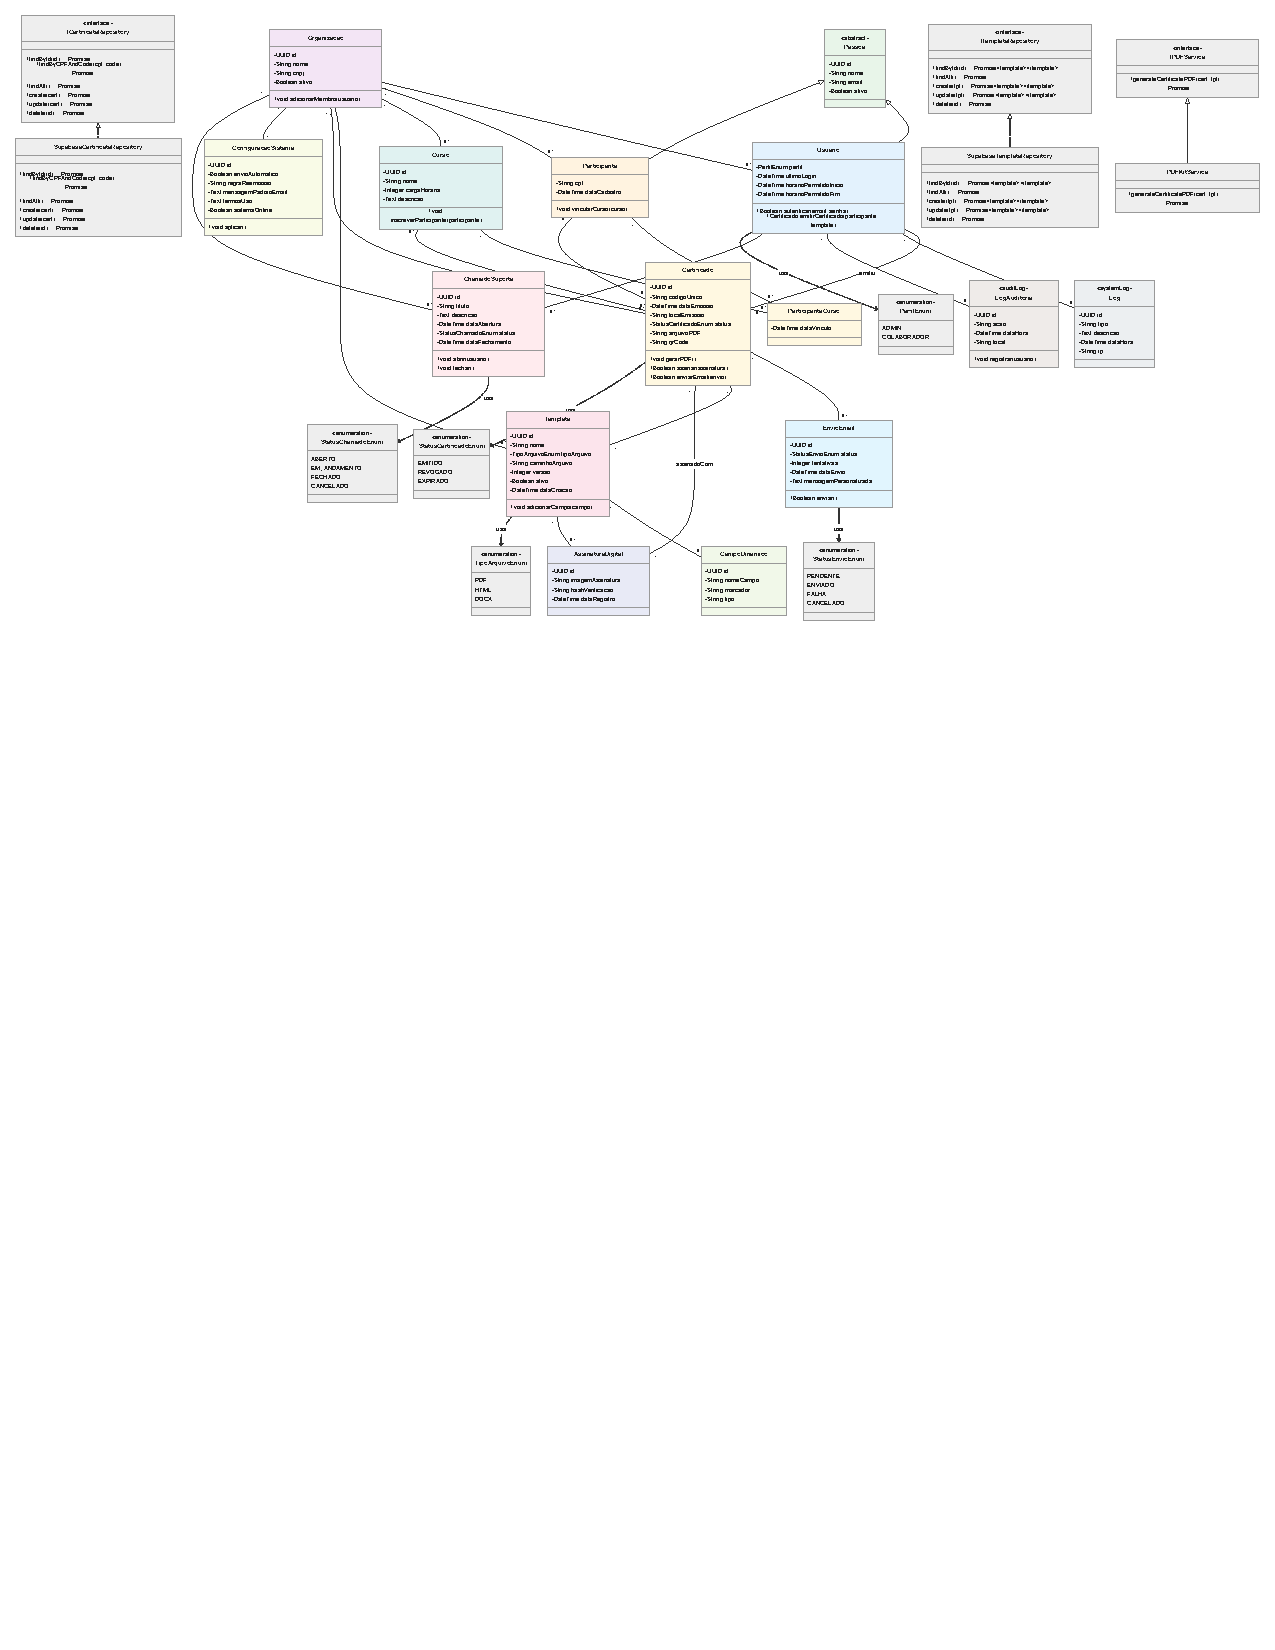
\includegraphics[width=0.9\textwidth]{imagens/diagrama-de-classes.pdf}
    \caption{Diagrama de Classes --- Sistema de Certificados}
    \label{fig:diagrama-classes}
\end{figure}



\subsection{Arquitetura do Sistema}

A arquitetura do sistema foi projetada para atender aos requisitos de independência entre camadas, testabilidade e facilidade de manutenção. Optou-se por uma abordagem de duas aplicações independentes --- frontend e backend --- que se comunicam exclusivamente via API REST. Essa separação permite que cada aplicação seja desenvolvida, testada, implantada e escalada de forma independente, sem acoplamento tecnológico entre as camadas de apresentação e lógica de negócio.

O backend adota uma arquitetura em quatro camadas, organizadas pelo princípio de inversão de dependências, em que camadas externas dependem de camadas internas:

\begin{enumerate}
    \item \textbf{Apresentação (\textit{App})} --- \textit{Route Handlers} do Next.js que expõem os endpoints REST (\code{/api/certificates}, \code{/api/templates}, \code{/api/verify}) e o utilitário \texttt{handle\-Api\-Error}, que converte exceções de domínio e erros de validação Zod em respostas HTTP padronizadas. Esta camada recebe a requisição, faz o \textit{parse} do JSON, aciona a validação do DTO e delega a execução ao \textit{use case}.
    \item \textbf{Aplicação (\textit{Application})} --- \textit{Use cases} que orquestram o fluxo de negócio (Emitir, Listar, Verificar, Gerar PDF, Gerenciar Templates) e \textbf{DTOs} definidos como esquemas Zod (\code{EmitCertificateDTO}, \code{UpdateValidityDTO}, \code{VerifyCertificateDTO}, etc.), que validam os dados de entrada antes de alcançarem o domínio.
    \item \textbf{Domínio (\textit{Domain})} --- Núcleo da aplicação, sem dependências externas. Contém as \textbf{entidades} (\code{Certificate}, \code{Template}) com suas regras de negócio encapsuladas, \textbf{interfaces de repositório} (\code{ICertificateRepository}, \code{ITemplateRepository}), \textbf{interfaces de serviço} (\code{IPDFService}), \textbf{\textit{Value Objects}} (\code{VerificationCode}, com geração e validação de código único) e \textbf{erros de domínio} (\code{CertificateNotFoundError}, \code{InvalidCertificateDataError}, etc.).
    \item \textbf{Infraestrutura (\textit{Infrastructure})} --- Implementações concretas das interfaces definidas no domínio: \code{SupabaseCertificateRepository}, \code{SupabaseTemplateRepository} e \code{PDFKitService}, além dos clientes de acesso ao banco PostgreSQL gerenciado pelo Supabase.
\end{enumerate}

O fluxo de dados percorre as camadas da seguinte forma: uma requisição HTTP chega ao \textit{Route Handler} (Apresentação), que valida o corpo da requisição contra o esquema Zod (Aplicação) e invoca o \textit{use case}. O \textit{use case} orquestra as operações de negócio utilizando entidades e \textit{Value Objects} do Domínio, e persiste os dados por meio das interfaces de repositório --- cujas implementações concretas (Infraestrutura) são injetadas via construtor. A resposta segue o caminho inverso até ser retornada ao cliente. Esse isolamento garante que as regras de negócio permaneçam independentes de frameworks, bancos de dados ou serviços externos. A inversão de dependência é obtida por meio de interfaces definidas no domínio e implementadas na infraestrutura --- por exemplo, \code{ICertificateRepository} e \code{IPDFService} são contratos que o \textit{use case} de emissão consome sem conhecer a implementação concreta. Entre as limitações desta abordagem, destaca-se o aumento do número de arquivos e interfaces, o que pode elevar a complexidade inicial do projeto em comparação com arquiteturas mais simples como \textit{controllers} monolíticos.

O frontend adota uma arquitetura em camadas com React, composta por quatro camadas que separam responsabilidades de forma clara. A \textbf{View} (apresentação) contém os componentes React que renderizam a interface do usuário, divididos em páginas (\code{views/}) e componentes reutilizáveis (\code{components/}), incluindo os do shadcn/ui. A \textbf{ViewModel} (lógica de apresentação) é formada por custom hooks (\code{useCertificatesViewModel}, \code{useDashboardViewModel}, etc.) que encapsulam estado (\code{useState}), efeitos colaterais (\code{useEffect}) e dados derivados (\code{useMemo}), expondo um objeto com estado e manipuladores para a camada View. O \textbf{Service} (infraestrutura) centraliza a comunicação com o backend: o módulo \code{api.ts} consome a API REST via \code{fetch}, e o módulo \code{envios.ts} gerencia a fila local de envios de e-mail no \code{localStorage} --- armazenando apenas dados operacionais (nome e e-mail do destinatário, \textit{status} da entrega), sem tokens de autenticação ou credenciais. O \textbf{Model} (domínio) reúne as interfaces TypeScript que definem as entidades do sistema (\code{Certificate}, \code{Template}, \code{VerifyResult}, \code{EnvioEmail}). O TanStack Router orquestra a navegação entre as Views, e o Tailwind CSS gerencia a estilização em todas as camadas de apresentação. Essa separação permite testar a lógica de apresentação independentemente da interface, utilizando Jest para validar os ViewModels sem depender de um navegador. Como limitação, o aumento do número de ViewModels eleva a quantidade de arquivos e hooks, o que pode tornar a navegação entre camadas mais custosa em projetos de grande escala.

O fluxo de comunicação entre as duas aplicações ocorre da seguinte forma: o frontend SPA, executado no navegador, faz requisições HTTPS aos \textit{Route Handlers} do backend por meio do módulo \code{api.ts} (camada Service), que encapsula a \code{fetch} API nativa. As requisições são autenticadas via token JWT gerenciado pelo Supabase Auth e trafegam sobre HTTPS (TLS 1.2), conforme RNF044. O backend processa a requisição através de suas quatro camadas --- Apresentação, Aplicação, Domínio e Infraestrutura --- e retorna a resposta padronizada ao frontend. Esse fluxo ponta a ponta está representado nos diagramas das Figuras~\ref{fig:backend} e~\ref{fig:frontend}, onde a seta "HTTPS REST + JWT" conecta o frontend SPA aos \textit{Route Handlers} do backend.

\begin{figure}[H]
    \centering
    \caption{Arquitetura do Backend — Quatro camadas (App, Application, Domain, Infrastructure) com DTOs, Value Objects e fluxo de dependências}
    \label{fig:backend}
    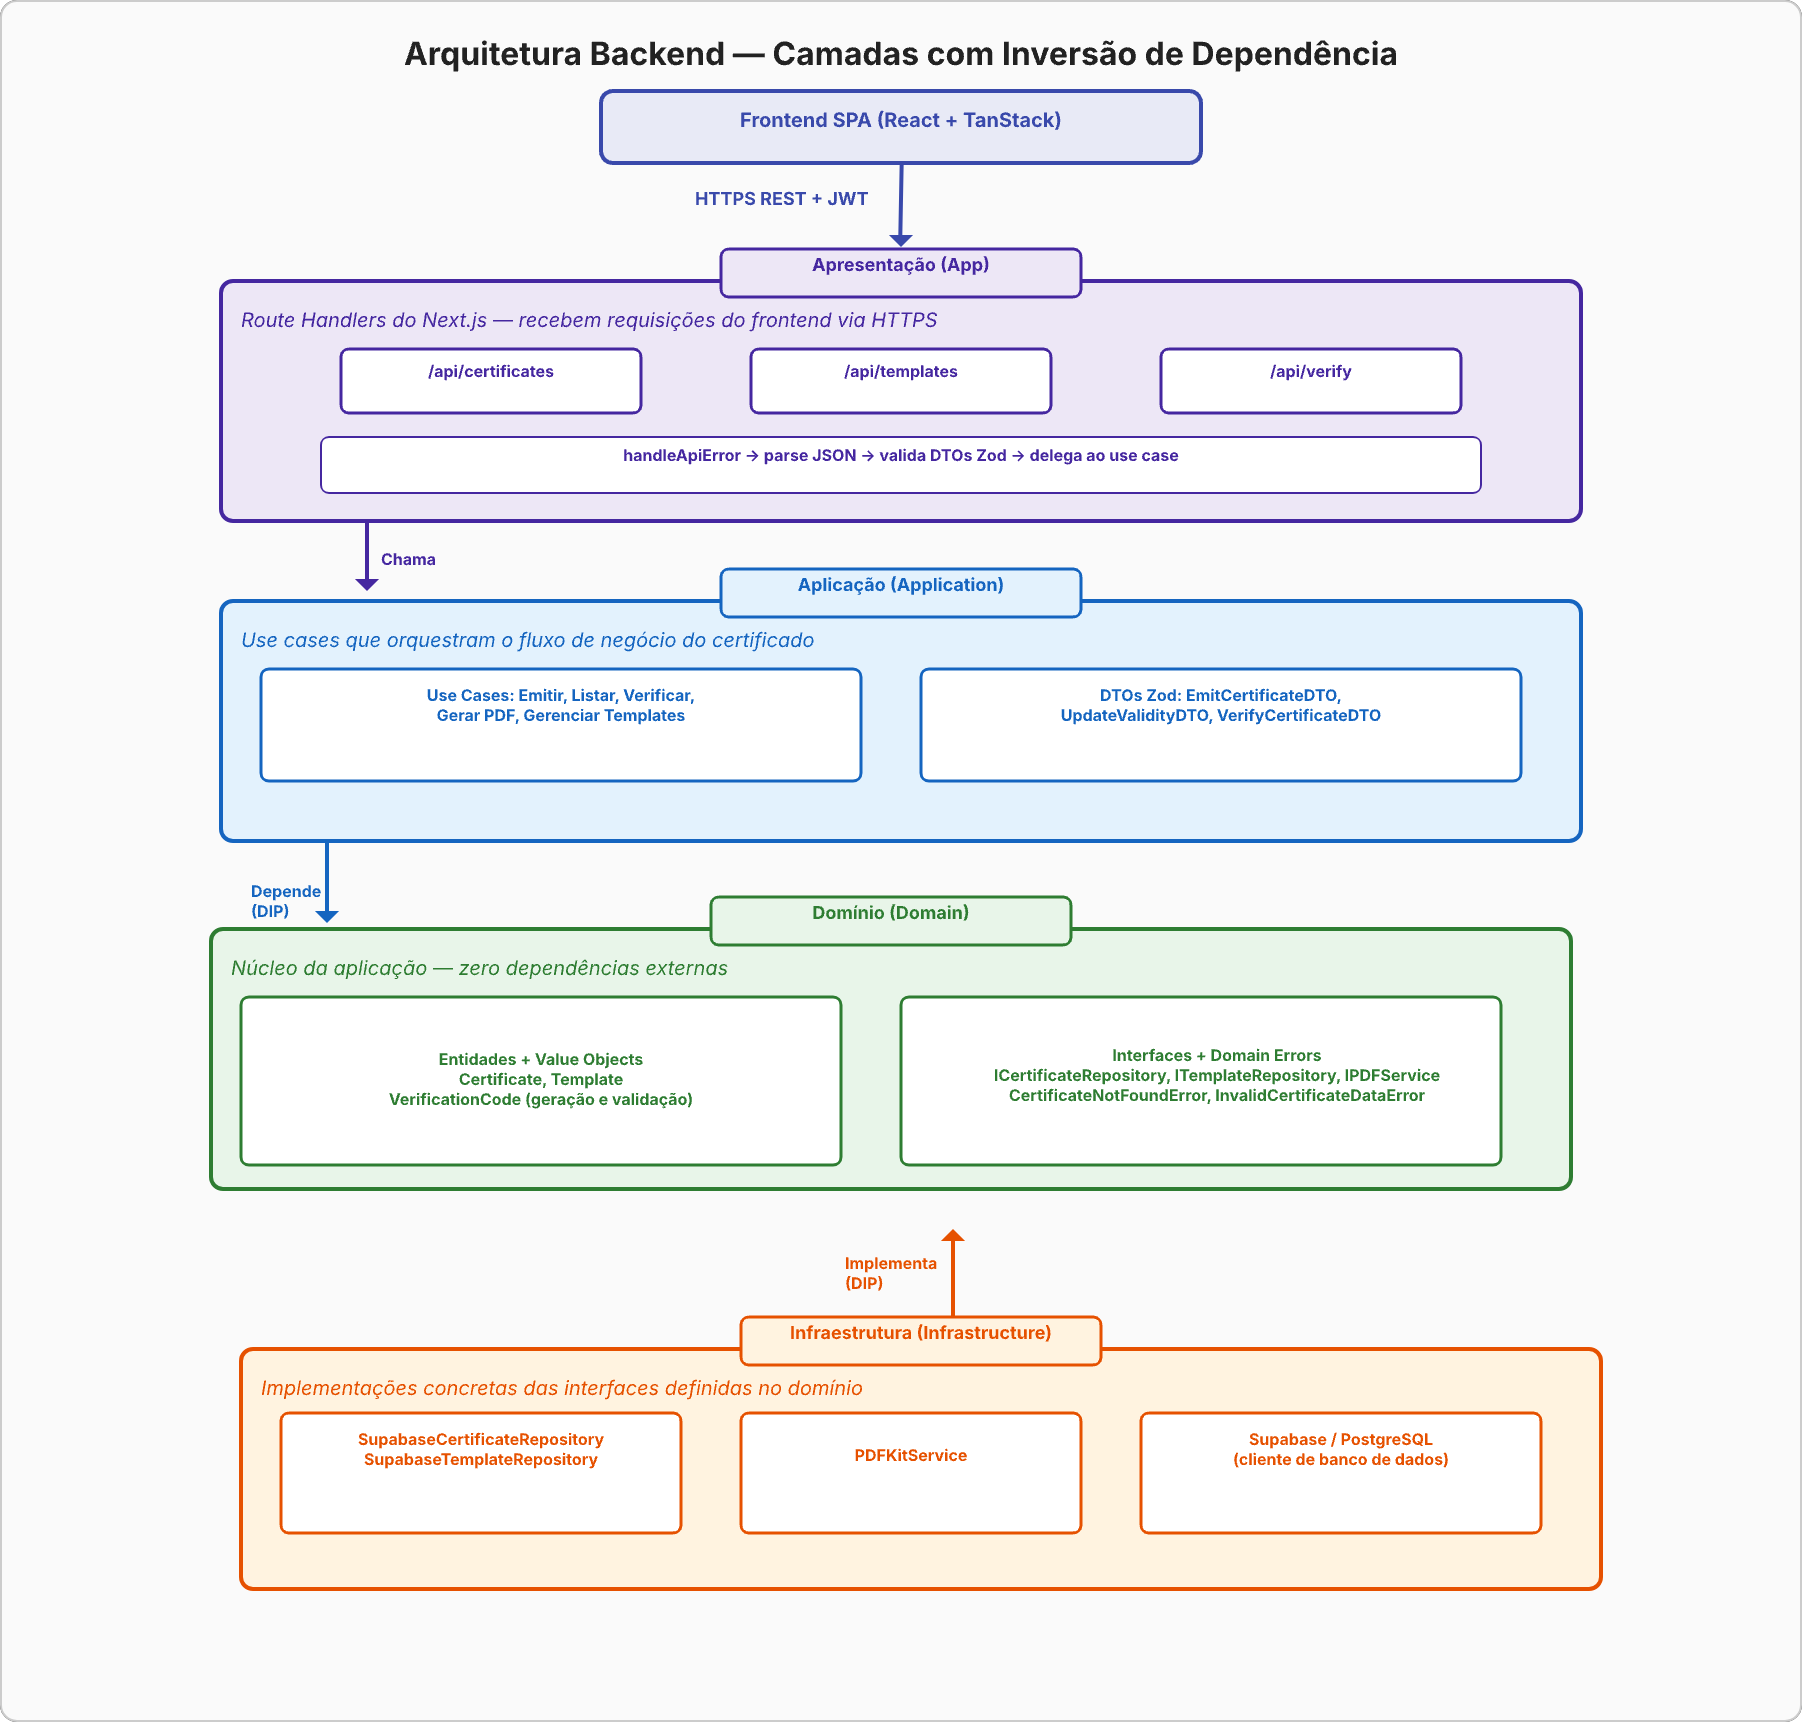
\includegraphics[width=0.9\textwidth]{imagens/backend.png}
    \par\vspace{0.5em}
    \parbox{\textwidth}{\raggedright\small\textit{Fonte: Elaborado pelo Autor (2026).}}
\end{figure}


\begin{figure}[H]
    \centering
    \caption{Arquitetura do Frontend — Quatro camadas (View, ViewModel, Service, Model) com React}
    \label{fig:frontend}
    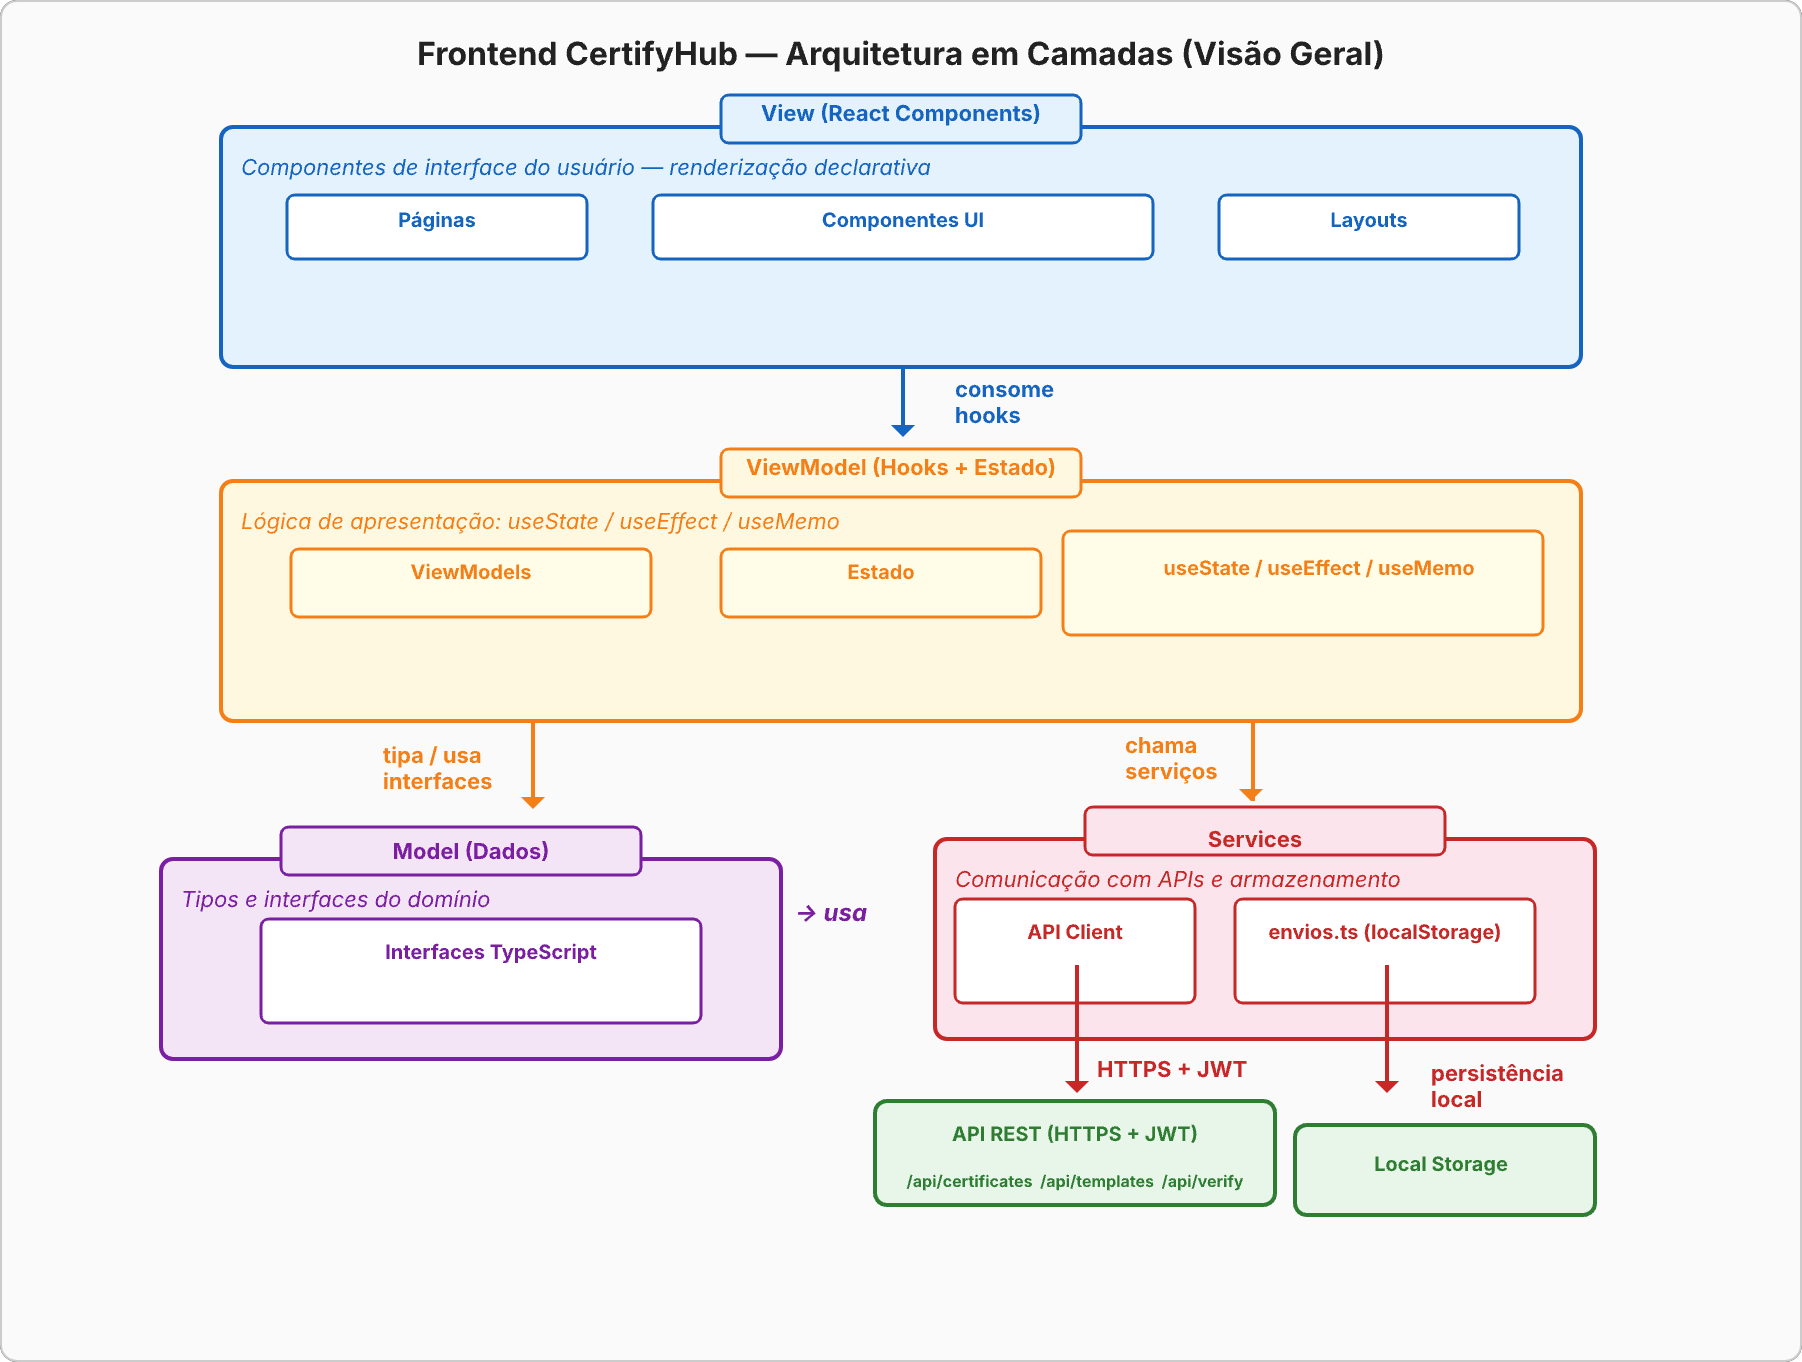
\includegraphics[width=0.9\textwidth]{imagens/frontend.png}
    \par\vspace{0.5em}
    \parbox{\textwidth}{\raggedright\small\textit{Fonte: Elaborado pelo Autor (2026).}}
\end{figure}


\subsection{Diagrama Entidade-Relacionamento}
O Diagrama Entidade-Relacionamento da Figura~\ref{fig:der} modela a estrutura do banco de dados implementada no MVP do sistema, composta por duas entidades principais: \code{CERTIFICADOS} e \code{TEMPLATES}. A notação adotada é a pé-de-galinha (Engenharia da Informação), onde o símbolo de barra (---) indica o lado ``1'' e o símbolo de três pontas (--<) indica o lado ``N'' (muitos). Ambas as entidades utilizam UUID como identificador primário.

A entidade \code{CERTIFICADOS} armazena os certificados emitidos e contém os seguintes atributos: \code{id} (PK, UUID), \code{recipientName} (varchar 200, NOT NULL), \code{recipientCPF} (varchar 11, NOT NULL, indexado), \code{courseName} (varchar 300, NOT NULL), \code{courseHours} (integer, NOT NULL), \code{verificationCode} (varchar 8, UNIQUE, NOT NULL), \code{validityDate} (timestamptz, NOT NULL), \code{templateId} (FK, UUID, NOT NULL), \code{issuedAt} (timestamptz, NOT NULL), \code{createdAt} (timestamptz, NOT NULL) e \code{updatedAt} (timestamptz, NOT NULL).

A entidade \code{TEMPLATES} gerencia os modelos de certificado disponíveis para emissão, com os atributos: \code{id} (PK, UUID), \code{name} (varchar 100, NOT NULL), \code{description} (text), \code{layoutConfig} (jsonb), \code{createdAt} (timestamptz, NOT NULL) e \code{updatedAt} (timestamptz, NOT NULL).

O relacionamento entre as entidades é de 1:N (um template pode ser usado por vários certificados), materializado pela chave estrangeira \code{templateId} na entidade \code{CERTIFICADOS} que referencia \code{TEMPLATES(id)}. Essa modelagem reflete o escopo reduzido do MVP, que contempla exclusivamente as funcionalidades de emissão de certificados com suporte a templates personalizáveis, sem as entidades de usuários, organizações, participantes, cursos e auditoria que serão incorporadas em versões futuras do sistema.

Vale ressaltar que, no estado atual do sistema, as informações relativas a participantes e cursos são armazenadas de forma denormalizada diretamente na entidade \code{CERTIFICADOS}, por meio dos atributos \code{recipientName}, \code{recipientCPF}, \code{courseName} e \code{courseHours}. Essa abordagem elimina a necessidade de chaves estrangeiras para entidades de participantes e cursos, simplificando a implementação do MVP, porém introduz redundância de dados e compromete a integridade referencial. Em versões futuras, as entidades \code{PARTICIPANTES} e \code{CURSOS} serão materializadas no banco de dados, permitindo a associação por meio de chaves estrangeiras (\code{participantId} e \code{courseId}), eliminando a duplicação de dados e habilitando funcionalidades como histórico de certificados por participante, listagem de certificados por curso e relatórios gerenciais por unidade de treinamento.

O Diagrama de Classes (Figura~\ref{fig:diagrama-classes}) apresenta a hierarquia \code{PESSOA} $\rightarrow$ \code{USUARIO} / \code{PARTICIPANTE} como uma generalização conceitual oriunda do modelo de domínio. No banco de dados físico do MVP, essas entidades não foram materializadas --- apenas \code{CERTIFICADOS} e \code{TEMPLATES} existem como tabelas. A implementação futura dessa herança seguirá a estratégia \textit{joined-table} (ou \textit{table-per-type}), na qual \code{PESSOA} seria uma tabela concreta com os atributos comuns (\code{id}, \code{nome}, \code{email}) e cada subtipo (\code{USUARIO}, \code{PARTICIPANTE}) teria sua própria tabela com chave primária que é também chave estrangeira referenciando \code{PESSOA(id)} --- garantindo integridade referencial sem armazenamento redundante.

\begin{figure}[H]
    \centering
    \caption{Diagrama Entidade-Relacionamento (DER) --- MVP do Banco de Dados}
    \label{fig:der}
    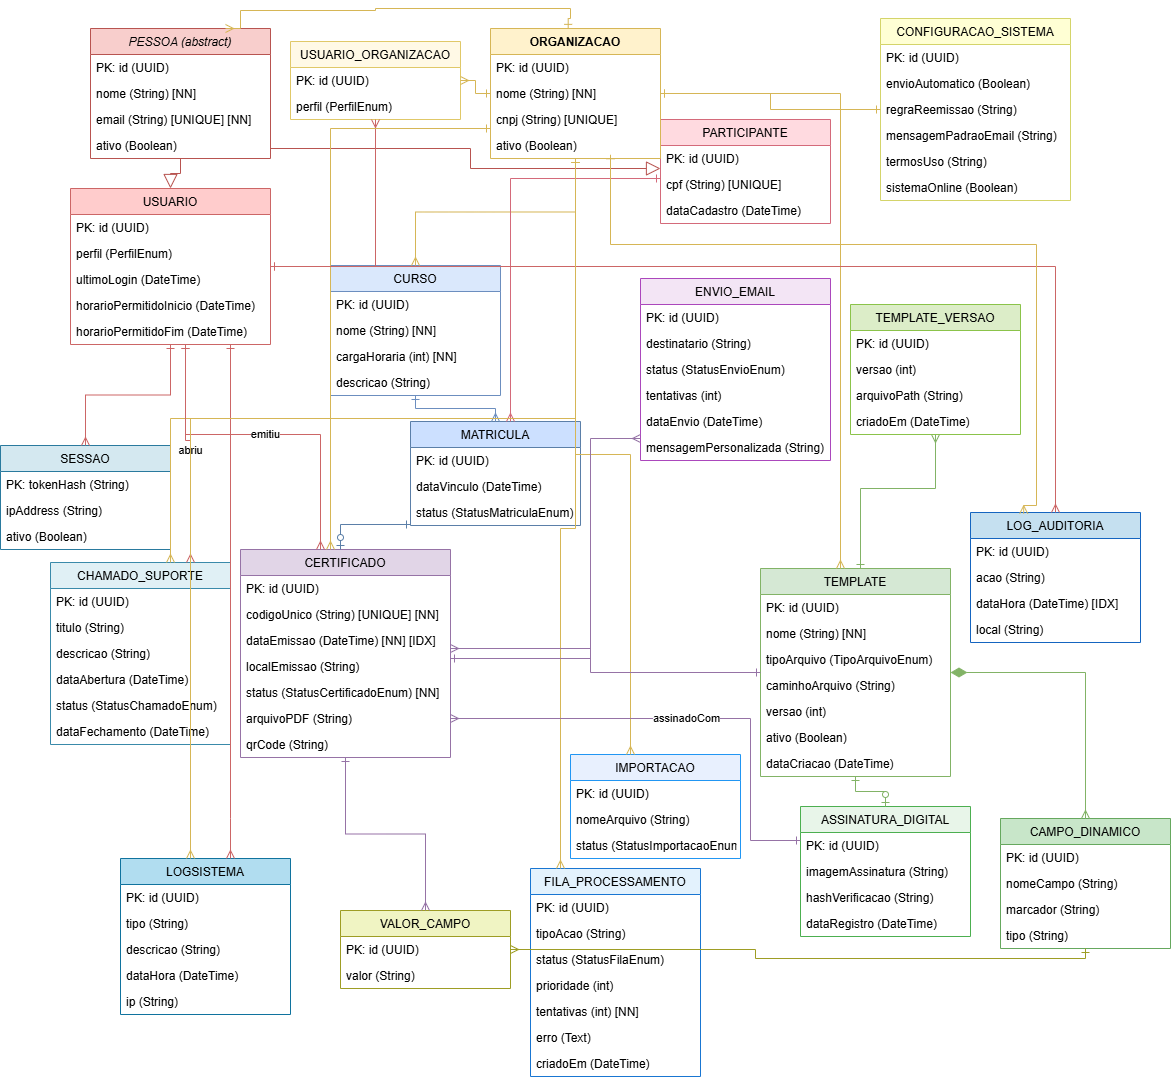
\includegraphics[width=0.9\textwidth]{imagens/DER.png}
\end{figure}

\subsection{Interfaces}
\begin{figure}[H]
    \centering
    
\includegraphics[width=\textwidth]{imagens/interface.png}
    \caption{Interface do Sistema --- Dashboard de Certificados}
    \label{fig:interface}
\end{figure}

